% ថ្នាក់ទី ១១ (វិទ្យាសាស្ត្រសង្គម) · ជំពូកទី ៦ · មេរៀនទី ១ · សៀវភៅ ទំព័រ ២១៣–២២៧
\chapter{ចម្លាស់}

\begin{note}[ជំពូកទី ៦ ៖ ចម្លាស់ បន្សំ និងប្រូបាប]
សួនសត្វមួយមានច្រកសម្រាប់ចេញចូលបួន ។ ភ្ញៀវអាចចេញចូលតាមច្រកមួយណាក៏បាន ។ តែមិនអាចចេញមកវិញតាមច្រកដែលបានចូលទេ ។ បើពួសុខគាត់ចូលច្រក ① នោះគាត់អាចចេញតាមច្រក ②, ③ ឬទី ④ មានន័យថា គាត់មាន $3$ របៀបក្នុងការចេញ ។ តាមរបៀបនេះ តើអ្នកដឹងថា មានប៉ុន្មានរបៀបក្នុងការចូលទៅទស្សនា និងចេញមកវិញ? តើគេអាចប៉ាន់ស្មានសំណាងដែលគេចេញមកវិញតាមច្រកទី ① មានតម្លៃប៉ុន្មាន?
\end{note}

\begin{objBox}[វត្ថុបំណង]
\begin{enumerate}[1]
  \item រាប់ចំនួនលទ្ធផលដែលកើតឡើងក្នុងវិញ្ញាសាមួយ
  \item រកចំនួនលទ្ធផលនៃព្រឹត្តិការណ៍ $2$ កើតឡើង
  \item សង់ដ្យាក្រាមដើមឈើ
  \item តម្រៀបធាតុ សង់ដ្យាក្រាមដើមឈើ
  \item រកចំនួនចម្លាស់នៃ $n$ ធាតុ
  \item រកចំនួនចម្លាស់នៃ $r$ ធាតុយកពី $n$ ធាតុ
  \item រកចំនួនចម្លាស់ច្រំដែល
  \item រកចំនួនចម្លាស់វង់ ។
\end{enumerate}
\end{objBox}

\section{គោលការណ៍រាប់}
\subsection{គោលការណ៍ផលបូក}

\begin{example}[ឧទាហរណ៍ ១]
គេបោះគ្រាប់ឡុកឡាក់ពីរគ្រាប់មានទំហំខុសគ្នាគឺមួយតូច មួយធំ ។ ចំនួនដែលបង្ហាញនៅមុខខាងលើនៃគ្រាប់ឡុកឡាក់ទាំងពីរហៅថា \textbf{លទ្ធផលមួយ} ។ តើគេបានលទ្ធផលប៉ុន្មានរបៀប បើចំនួននៅមុខលើនៃគ្រាប់ឡុកឡាក់ទាំងពីរមានផលបូកស្មើនឹង $3$ ឬ $4$?
\end{example}
ផលបូកស្មើ $3$ អាចសរសេរ $3 = 1 + 2 = 2 + 1$ ។ ផលបូកស្មើ $4$ អាចសរសេរ $4 = 1 + 3 = 2 + 2 = 3 + 1$ ។
\begin{itemize}
  \item លទ្ធផលដែលមានផលបូកស្មើនឹង $3$ មានគូលំដាប់ $(1, 2)$ និង $(2, 1)$ ។
  \item លទ្ធផលដែលមានផលបូកស្មើនឹង $4$ មានគូលំដាប់ $(1, 3)$, $(2, 2)$ និង $(3, 1)$ ។
  \item គេឃើញថាក្នុងករណីទាំងពីរនេះគ្មានលទ្ធផលណាមួយដូចគ្នាទេ ។ គេបានចំនួនលទ្ធផលដែលកើតឡើងទាំងអស់គឺ $2 + 3 = 5$ ។
\end{itemize}
បើគេតាង $A$ ជាព្រឹត្តិការណ៍ដែលគ្រាប់ឡុកឡាក់ទាំងពីរចេញគូចំនួនដែលមានផលបូកស្មើនឹង $3$ នោះចំនួនលទ្ធផលដែលកើតក្នុងព្រឹត្តិការណ៍ $A = \{(1, 2), (2, 1)\}$ មាន $2$ របៀប ។ គេកំណត់សរសេរ $n(A) = 2$ ។ បើ $B = \{(1, 3), (2, 2), (3, 1)\}$ ជាព្រឹត្តិការណ៍ដែលគ្រាប់ឡុកឡាក់ទាំងពីរមានផលបូកស្មើនឹង $4$ នោះ $n(B) = 3$ ។

គេបានព្រឹត្តិការណ៍ដែលគ្រាប់ឡុកឡាក់មានផលបូកស្មើនឹង $3$ ឬ $4$ គឺជាព្រឹត្តិការណ៍ $A$ ឬ $B$ ។ គេកំណត់សរសេរ $A \cup B = \{(1, 2), (2, 1), (1, 3), (2, 2), (3, 1)\}$ ។ ដោយព្រឹត្តិការណ៍ $A$ និងព្រឹត្តិការណ៍ $B$ គ្មានលទ្ធផលណាមួយដូចគ្នា នោះចំនួនលទ្ធផលដែលកើតក្នុងព្រឹត្តិការណ៍ $A$ ឬ $B$ គឺ $n(A \cup B) = n(A) + n(B) = 2 + 3 = 5$ ។

\begin{example}[ឧទាហរណ៍ ២]
គេធ្វើពិសោធន៍ដូចក្នុងឧទាហរណ៍ $1$ ហើយគេចង់ដឹងថា តើលទ្ធផលមានប៉ុន្មានរបៀប បើគ្រាប់ឡុកឡាក់ទាំងពីរមានផលបូកស្មើនឹង $4$ ឬផលគុណស្មើនឹង $4$?
\end{example}
ផលបូកស្មើ $4$ អាចសរសេរ $4 = 1 + 3 = 2 + 2 = 3 + 1$ (ព្រោះគ្រាប់ឡុកឡាក់មានតែលេខ $1, 2, 3, 4, 5$ និង $6$ ប៉ុណ្ណោះ) ។
\begin{itemize}
  \item លទ្ធផលដែលមានផលបូកស្មើនឹង $4$ មានគូលំដាប់ $(1, 3)$, $(2, 2)$ និង $(3, 1)$ ។
  \item លទ្ធផលដែលមានផលគុណស្មើនឹង $4$ មានគូលំដាប់ $(1, 4)$, $(2, 2)$ និង $(4, 1)$ ។
  \item គេឃើញថា ចំនួនលទ្ធផលដែលគ្រាប់ឡុកឡាក់ទាំងពីរមានផលបូកស្មើនឹង $4$ ឬផលគុណស្មើនឹង $4$ មិនអាចស្មើនឹង $3 + 3 = 6$ របៀបទេ ព្រោះក្នុងករណីទាំងពីរនេះ មានលទ្ធផលរួមគ្នាមួយគឺ មានលំដាប់ $(2, 2)$ ។
  \item បើគេតាង $C$ ជាព្រឹត្តិការណ៍ដែលគ្រាប់ឡុកឡាក់ទាំងពីរមានផលគុណស្មើនឹង $4$ ហើយ $B$ ជាព្រឹត្តិការណ៍ដែលគ្រាប់ឡុកឡាក់ទាំងពីរមានផលបូកស្មើនឹង $4$ ។
  \item គេបានគូលំដាប់ $(2, 2)$ គឺជាលទ្ធផលនៃព្រឹត្តិការណ៍ $B$ និង $C$ ដែលគេកំណត់សរសេរដោយ $B \cap C$ ដែលមានចំនួនលទ្ធផល $n(B \cap C) = 1$ ។ ដូច្នេះចំនួនលទ្ធផលនៃព្រឹត្តិការណ៍ $B \cup C$ គឺ $n(B \cup C) = n(B) + n(C) - n(B \cap C) = 3 + 3 - 1 = 5$ ។
\end{itemize}

\begin{formulaBox}[ជាទូទៅ]
គេមានព្រឹត្តិការណ៍ $A$ និងព្រឹត្តិការណ៍ $B$ ។ $n(A)$ ជាចំនួនលទ្ធផលកើតក្នុងព្រឹត្តិការណ៍ $A$ ។ $n(B)$ ជាចំនួនលទ្ធផលកើតក្នុងព្រឹត្តិការណ៍ $B$ ។
\begin{itemize}
  \item បើ $A$ និង $B$ ជាពីរព្រឹត្តិការណ៍ពីរមិនចុះសម្រុងគ្នា (គ្មានលទ្ធផលណាមួយរួមទេ) នោះចំនួនលទ្ធផលដែលកើតឡើងក្នុងព្រឹត្តិការណ៍ «$A$ ឬ $B$» គឺ $n(A \cup B) = n(A) + n(B)$ ។
  \item បើ $A$ និង $B$ ជាព្រឹត្តិការណ៍ពីរចុះសម្រុងគ្នា (មានលទ្ធផលរួមគ្នា) នោះចំនួនលទ្ធផលដែលកើតឡើងក្នុងព្រឹត្តិការណ៍ «$A$ ឬ $B$» គឺ $n(A \cup B) = n(A) + n(B) - n(A \cap B)$ ។
\end{itemize}
\end{formulaBox}

\begin{pro}
\begin{enumerate}[1]
  \item គេបោះគ្រាប់ឡុកឡាក់ពីរគ្រាប់ មួយពណ៌ស មួយទៀតពណ៌ក្រហម ។ រកចំនួនលទ្ធផលដែលកើតឡើង កាលណាលទ្ធផលមានផលបូកលេខស្មើនឹង $5$ ឬ $6$ ។
  \item ក្នុងថង់មួយមានប័ណ្ណ $6$ ដែលបង់លេខ $1, 2, 3, 4, 5, 6$ ។ គេចាប់យកប័ណ្ណមួយចេញពីថង់ដោយចៃដន្យ ។ រកចំនួនលទ្ធផលដែលអាចកើតឡើង កាលណាលេខដែលចាប់បានជាលេខសេស ឬលេខធំជាង $4$ ។
\end{enumerate}
\ans
\begin{enumerate}[1]
  \item $4 + 5 = 9$
  \item $\{1, 3, 5\} \cup \{5, 6\} = \{1, 3, 5, 6\}$ ដូច្នេះមាន $3 + 2 - 1 = 4$ ។
\end{enumerate}
\end{pro}

\subsection{គោលការណ៍ផលគុណ}

\begin{example}[ឧទាហរណ៍ ១]
គេមានអាវ $4$ និងខោ $3$ ផ្សេងៗគ្នា ។ តើគេអាចស្លៀកពាក់បានប៉ុន្មានរបៀបខុសៗគ្នា បើគេចាប់យកអាវ $1$ និងខោ $1$ ដោយចៃដន្យក្នុងចំណោមអាវ $4$ និងខោ $3$ នេះមកប្រើ ។
\end{example}
\begin{itemize}
  \item គេអាចរាប់បានថា បើគេរើសយកអាវមួយទៅប្រើជាមួយខោណាមួយក្នុងចំណោមខោ $3$ នោះគេបានសម្លៀកបំពាក់ $3$ របៀបខុសៗគ្នា ។
  \item បើគេប្រើអាវ $4$ និងខោ $3$ នោះគេបានសម្លៀកបំពាក់ $4$ ដងច្រើនជាង គឺ $4\times 3 = 12$ របៀបខុសៗគ្នា ។
\end{itemize}
ដូច្នេះ គេអាចជ្រើសរើសអាវ $1$ និងខោ $1$ ក្នុងចំណោមអាវ $4$ និងខោ $3$ មកស្លៀកពាក់បាន $12$ របៀប ។ ដើម្បីបង្ហាញការរាប់ឱ្យកាន់តែច្បាស់ គេប្រើដ្យាក្រាមដើមឈើ ៖

\begin{center}
\begin{tikzpicture}[scale=0.85]
  \node[draw,circle,inner sep=1.5pt] (r) at (0,0) {};
  \foreach \i/\x in {1/-5.4,2/-1.8,3/1.8,4/5.4} {
    \node[draw,rounded corners,font=\small,fill=blue!8] (a\i) at (\x,-1.4) {អាវ\,$\i$};
    \draw (r) -- (a\i);
    \foreach \j/\d in {1/-1.1,2/0,3/1.1} {
      \node[draw,font=\scriptsize,fill=orange!10,inner sep=2pt] (b\i\j) at (\x+\d,-2.9) {ខោ\,$\j$};
      \draw (a\i) -- (b\i\j);
    }
  }
\end{tikzpicture}
\end{center}

\begin{itemize}
  \item តាង $A$ ជាព្រឹត្តិការណ៍ចាប់យកអាវ $1$ ដោយចៃដន្យក្នុងចំណោមអាវ $4$ គេបានចំនួនលទ្ធផល $n(A) = 4$ ។
  \item តាង $B$ ជាព្រឹត្តិការណ៍ចាប់យកខោ $1$ ដោយចៃដន្យក្នុងចំណោមខោ $3$ គេបានចំនួនលទ្ធផល $n(B) = 3$ ។
\end{itemize}
ដូច្នេះ ចំនួនលទ្ធផលនៃព្រឹត្តិការណ៍ $A$ និងព្រឹត្តិការណ៍ $B$ កើតឡើងបន្តបន្ទាប់គ្នាស្មើនឹង $n(A)\times n(B) = 4\times 3 = 12$ របៀប ។

\begin{formulaBox}[ជាទូទៅ]
គេមានព្រឹត្តិការណ៍ $A$ កើតឡើង $m$ របៀប ហើយមានព្រឹត្តិការណ៍ $B$ កើតឡើង $n$ របៀប នោះចំនួនលទ្ធផលដែលព្រឹត្តិការណ៍ $A$ កើតឡើង ហើយ $B$ កើតឡើងបន្ទាប់ស្មើនឹង $m\times n$ ។
\end{formulaBox}

\begin{example}[លំហាត់គំរូ]
គេមានផ្លូវ $3$ ខ្សែសម្រាប់ធ្វើដំណើរពីក្រុង $A$ ទៅ $B$ និងមានផ្លូវ $2$ ខ្សែសម្រាប់ធ្វើដំណើរពីក្រុង $B$ ទៅក្រុង $C$ ។ តើគេអាចធ្វើដំណើរតាមផ្លូវបានប៉ុន្មានរបៀប ដើម្បីចេញពីក្រុង $A$ ទៅ $C$ ដោយឆ្លងកាត់តាមក្រុង $B$ ។
\end{example}
\ans
\begin{center}
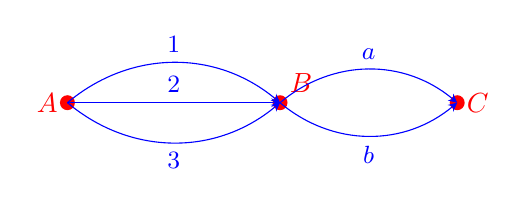
\begin{tikzpicture}[scale=0.9,>=stealth]
  \fill[red] (0,0) circle (3pt) node[left] {$A$};
  \fill[red] (3,0) circle (3pt) node[above right] {$B$};
  \fill[red] (5.5,0) circle (3pt) node[right] {$C$};
  \draw[->,blue] (0,0) to[bend left=40] node[above] {\small $1$} (3,0);
  \draw[->,blue] (0,0) -- node[above] {\small $2$} (3,0);
  \draw[->,blue] (0,0) to[bend right=40] node[below] {\small $3$} (3,0);
  \draw[->,blue] (3,0) to[bend left=40] node[above] {\small $a$} (5.5,0);
  \draw[->,blue] (3,0) to[bend right=40] node[below] {\small $b$} (5.5,0);
\end{tikzpicture}
\end{center}
តាង $1, 2, 3$ ជាផ្លូវភ្ជាប់ពីក្រុង $A$ ទៅ $B$ និង $a, b$ ជាផ្លូវភ្ជាប់ពីក្រុង $B$ ទៅក្រុង $C$ ។ ដើម្បីធ្វើដំណើរពី $A$ ទៅ $B$ គេមានផ្លូវ $3$ ជម្រើស និងផ្លូវពី $B$ ទៅ $C$ មាន $2$ ជម្រើស ។ តាមគោលការណ៍ផលគុណចំនួនរបៀបសម្រាប់ធ្វើដំណើរពី $A$ ទៅ $C$ ដោយឆ្លងកាត់តាម $B$ មាន $3\times 2 = 6$ របៀប ។

\begin{pro}
\begin{enumerate}[1]
  \item កំណត់ចំនួនស្លាកលេខ ដើម្បីសម្គាល់វត្ថុតាមប្រភេទដោយប្រើតួអក្សរមួយពី $A$ ដល់ $H$ សរសេរពីមុខលេខដែលប្រើលេខពី $1$ ដល់ $15$ ។
  \item មីងដានីចង់ទិញវត្ថុបីមុខមាន កាបូបដាក់សៀវភៅរៀនមួយ កាបូបតូចដាក់ប៊ិក ខ្មៅដៃមួយ និងល្បែងហ្គេមមួយឈុត សម្រាប់ជារង្វាន់លើកទឹកចិត្តកូនដែលបានជាប់ចំណាត់ថ្នាក់ល្អ ។ ពេលទៅដល់ហាងលក់វត្ថុទាំងនេះ គាត់ឃើញមានកាបូបដាក់សៀវភៅ $3$ ប្រភេទ $(A, B$ និង $C)$ កាបូបតូចមាន $4$ ពណ៌ (ក្រហម ខៀវ លឿង និងបៃតង) និងល្បែងហ្គេម $2$ ប្រភេទ $(I$ និង $II)$ ។ តើមីងដានីអាចជ្រើសរើសវត្ថុបីប្រភេទបានប៉ុន្មានរបៀប?
\end{enumerate}
\ans
\begin{enumerate}[1]
  \item $8\times 15 = 120$
  \item $3\times 4\times 2 = 24$ ។
\end{enumerate}
\end{pro}

\section{ចម្លាស់}
\subsection{ចម្លាស់នៃ \texorpdfstring{$n$}{n} ធាតុ}

\begin{example}[ឧទាហរណ៍]
គេមានប័ណ្ណ $4$ សន្លឹកចុះលេខ $6$, $7$, $8$ និង $9$ ។ បើគេយកប័ណ្ណនីមួយៗមកតម្រៀបជាជួរមានលំដាប់ នោះគេបានលទ្ធផលផ្សេងៗគ្នា ដែលជាចំនួនមាន $4$ លេខ ។ ចូរកំណត់ចំនួននៃចំនួនមាន $4$ លេខដែលបង្កើតបាន ។
\end{example}
ដើម្បីបានលទ្ធផលក្នុងការរៀបលេខទាំង $4$ នេះ គេត្រូវគិតពីការយកប័ណ្ណនីមួយៗមករៀបក្នុងការេ $4$ ៖ ខ្ទង់ទី $1$ អាចបាន $4$ របៀប (ព្រោះមាន $4$ ប័ណ្ណ), ខ្ទង់ទី $2$ អាចបាន $3$ របៀប (ព្រោះសល់ $3$ ប័ណ្ណ), ខ្ទង់ទី $3$ អាចបាន $2$ របៀប និងខ្ទង់ទី $4$ អាចបាន $1$ របៀប ។

\begin{center}
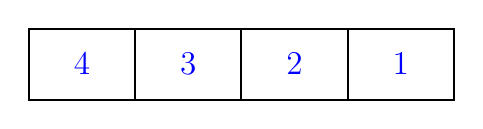
\begin{tikzpicture}[scale=0.9]
  \foreach \i/\v in {0/4,1/3,2/2,3/1} {
    \draw[thick] (\i*1.5,0) rectangle ++(1.5,1);
    \node[blue,font=\large] at (\i*1.5+0.75,0.5) {$\v$};
  }
\end{tikzpicture}
\end{center}

ដូច្នេះ តាមគោលការណ៍ផលគុណចំនួន នៃចំនួនមាន $4$ លេខដែលអាចកើតឡើងទាំងអស់មាន $4\times 3\times 2\times 1 = 24$ ។ ការតម្រៀបប័ណ្ណ $4$ សន្លឹកផ្សេងៗគ្នាតាម $4$ កន្លែងផ្សេងៗគ្នា ហើយគិតលំដាប់នេះហៅថាចម្លាស់នៃ $4$ ធាតុ ។ ចំនួនចម្លាស់នៃ $4$ ធាតុគឺ $4\times 3\times 2\times 1$ ឬគេកំណត់សរសេរដោយខ្លីគឺ $4!$ ($4!$ អានថា $4$ ហ្វាក់តូរីយ៉ែល ដែល $4! = 4\times 3\times 2\times 1$) ។ ដើម្បីបង្ហាញលទ្ធផលឱ្យកាន់តែច្បាស់ គេអាចបង្ហាញតាមដ្យាក្រាមដើមឈើ ។ លទ្ធផលទាំង $24$ គឺ ៖
\[
\begin{array}{cccccc}
6789 & 6798 & 6879 & 6897 & 6978 & 6987\\
7689 & 7698 & 7869 & 7896 & 7968 & 7986\\
8679 & 8697 & 8769 & 8796 & 8967 & 8976\\
9678 & 9687 & 9768 & 9786 & 9867 & 9876
\end{array}
\]

\begin{formulaBox}[ជាទូទៅ]
ចម្លាស់នៃ $n$ ធាតុ គឺជាតម្រៀបមានលំដាប់នៃ $n$ វត្ថុខុសៗគ្នាជាជួរដេក $n \in \mathbb{N}$ ។ ចំនួនចម្លាស់នៃ $n$ ធាតុស្មើនឹង $n!$ ។ $n!$ អានថា $n$ ហ្វាក់តូរីយ៉ែល
\[ n! = n(n - 1)(n - 2)\times\dots\times 4\times 3\times 2\times 1 \]
\end{formulaBox}

\begin{example}[លំហាត់គំរូ]
គ្រូធ្វើបញ្ជីឈ្មោះសិស្ស $8$ នាក់ដោយមានចុះលេខរៀងពី $1$ ដល់ $8$ តែមិនគិតតាមលំដាប់អក្ខរក្រមទេ ។
\begin{enumerate}[a]
  \item តើគ្រូអាចធ្វើបញ្ជីឈ្មោះបានប៉ុន្មានរបៀប?
  \item បើគ្រូចង់ឱ្យឈ្មោះសុក និងឈ្មោះសៅនៅជាប់គ្នា តើបញ្ជីឈ្មោះរបៀបនេះមានប៉ុន្មានបែប?
\end{enumerate}
\end{example}
\ans
\begin{enumerate}[a]
  \item ការសរសេរឈ្មោះតាមលំដាប់លេខរៀង គឺជាចម្លាស់ឈ្មោះសិស្ស $8$ នាក់ជាជួរ ។ ចំនួនចម្លាស់គឺ $8! = 8\times 7\times 6\times 5\times 4\times 3\times 2\times 1 = 40320$ ។ ដូច្នេះ គ្រូអាចធ្វើបញ្ជីឈ្មោះបាន $40320$ របៀប ។
  \item បើឈ្មោះសុក និងសៅនៅជាប់គ្នា គេចាត់ទុកថាឈ្មោះ $2$ នេះនៅក្នុងកន្លែងតែមួយ ម្យ៉ាងទៀតឈ្មោះសុក ឬសៅអាចនៅខាងមុខ ឬខាងក្រោយគ្នាគឺមាន $2$ របៀប បន្ទាប់មកគេត្រូវចម្លាស់សិស្ស $7$ នាក់ទៀត ។ ដូច្នេះ ចំនួនបញ្ជីឈ្មោះតាមបែបនេះមាន ៖ $2\times 7! = 2\times 7\times 6\times 5\times 4\times 3\times 2\times 1 = 10080$ របៀប ។
\end{enumerate}

\begin{pro}
\begin{enumerate}[1]
  \item គេរៀបសៀវភៅ $10$ ក្បាលខុសៗគ្នាដាក់ជាជួរលើធ្នើមួយ ។ ក. តើការតម្រៀបនេះមានប៉ុន្មានរបៀបខុសៗគ្នា? \quad ខ. បើគេកំណត់ឱ្យសៀវភៅ $3$ ក្បាលនៅជាប់គ្នាជានិច្ច តើការតម្រៀបនេះមានប៉ុន្មានបែប?
  \item មានមនុស្ស $6$ នាក់អង្គុយលើកៅអីមួយជួរដែលក្នុងនោះមានក្មេង $4$ នាក់ និងមនុស្សចាស់ $2$ នាក់ ។ រកចំនួនរបៀបការអង្គុយក្នុងករណីដែលមនុស្សចាស់ទាំង $2$ នាក់អង្គុយចុងសងខាង ។
\end{enumerate}
\ans
\begin{enumerate}[1]
  \item ក. $10! = 3628800$ \quad ខ. $3!\times 8! = 241920$
  \item $2!\times 4! = 48$ ។
\end{enumerate}
\end{pro}

\subsection{ចម្លាស់នៃ \texorpdfstring{$r$}{r} ធាតុយកពី \texorpdfstring{$n$}{n} ធាតុ}

\begin{example}[ឧទាហរណ៍]
គេបង្កើតលេខកូដមាន $4$ ខ្ទង់ខុសៗគ្នា ដើម្បីធ្វើប័ណ្ណពិសេសដោយប្រើ $6$ លេខ ៖ $0, 1, 3, 5, 7$ និង $9$ ។ តើគេអាចបង្កើតលេខកូដបានប៉ុន្មានប័ណ្ណ?
\end{example}
\begin{itemize}
  \item លេខកូដដែលអាចកើតឡើង គឺជាតម្រៀប $4$ លេខខុសៗគ្នាតាមលំដាប់ដែលលេខនីមួយៗយកចេញពី $6$ លេខ ។
  \item ដើម្បីសរសេរលេខខ្ទង់ដំបូង គេមាន $6$ លេខសម្រាប់ជ្រើសរើសយក $1$ លេខមកសរសេរក្នុងចំណោមលេខ $0, 1, 3, 5, 7$ និង $9$ ។
  \item លេខខ្ទង់ទី $2$ គេមាន $5$ លេខសម្រាប់ជ្រើសរើសយក $1$ លេខមកសរសេរ ព្រោះយើងប្រើអស់ $1$ លេខហើយ ។
  \item លេខខ្ទង់ទី $3$ គេមាន $4$ លេខសម្រាប់ជ្រើសរើសយក $1$ លេខ ព្រោះយើងប្រើអស់ $2$ លេខហើយ និងលេខប័ណ្ណខ្ទង់ចុងក្រោយ គេមាន $3$ លេខដែលនៅសល់ពីការសរសេរលេខ $3$ ខ្ទង់មុន សម្រាប់ជ្រើសរើសយក $1$ លេខ ។
\end{itemize}
ដោយសារយើងរើសលេខបន្តបន្ទាប់គ្នា ចំនួនលេខកូដទាំងអស់មាន $6\times 5\times 4\times 3 = 360$ ។ ការតម្រៀប $4$ លេខខុសគ្នាជាជួរមានលំដាប់ដែលលេខនីមួយៗយកចេញពី $6$ លេខខុសៗគ្នាហៅថា \textbf{ចម្លាស់នៃ $4$ ធាតុយកពី $6$ ធាតុ} ។ ចំនួនចម្លាស់នៃ $4$ ធាតុយកពី $6$ ធាតុគឺ
\[ 6\times 5\times 4\times 3 = \frac{6\times 5\times 4\times 3\times 2\times 1}{2\times 1} = \frac{6!}{2!} = \frac{6!}{(6 - 4)!} \]
គេកំណត់សរសេរ ${}_6P_4 = \dfrac{6!}{(6 - 4)!}$ ។

\begin{formulaBox}[ជាទូទៅ]
ចម្លាស់នៃ $r$ ធាតុយកចេញពី $n$ ធាតុ គឺជាតម្រៀបមានលំដាប់នៃ $r$ ធាតុខុសៗគ្នាដែលធាតុនីមួយៗយកចេញពី $n$ ធាតុខុសៗគ្នា $(n \in \mathbb{N}, r \in \mathbb{N}, r \le n)$ ។ ចំនួនចម្លាស់នៃ $r$ ធាតុយកចេញពី $n$ ធាតុគឺ
\[
\begin{gathered}
{}_nP_r = n(n - 1)(n - 2)\dots(n - r + 1) \quad \text{ឬ}\\
{}_nP_r = \frac{n!}{(n - r)!}
\end{gathered}
\]
គេអាចប្រើនិមិត្តសញ្ញា $P(n, r)$ ។
\end{formulaBox}

\begin{note}[សម្គាល់]
បើ $r = n$ នោះជាចម្លាស់នៃ $n$ ធាតុ ។ គេបាន ${}_nP_n = n!$ ព្រោះ $0! = 1$ ។
\end{note}

\begin{example}[លំហាត់គំរូ]
ក្នុងថង់មួយមានឃ្លី $7$ គ្រាប់ មានពណ៌ខុសៗគ្នា (ស ក្រហម ខៀវ លឿង ខ្មៅ បៃតង និងត្នោតចេក) ។ គេចាប់យកឃ្លីម្ដងមួយចេញពីថង់ រួចកត់ត្រាពណ៌ទុក ចំនួន $3$ ដងបន្តបន្ទាប់ដោយមិនដាក់ចូលថង់វិញ ក្រោយពីយកចេញពីថង់ម្ដងៗ ។
\begin{enumerate}[a]
  \item បើគេយកឃ្លីចេញតាមរបៀបនេះ តើគេបានលទ្ធផលប៉ុន្មានរបៀប?
  \item រកចំនួនលទ្ធផលដែលឃ្លីយកចេញលើកទី $2$ ជាឃ្លីពណ៌ក្រហម ។
\end{enumerate}
\end{example}
\ans
\begin{enumerate}[a]
  \item ការចាប់យកឃ្លី $3$ តាមរបៀបនេះ ជាការតម្រៀបឃ្លី $3$ តាមលំដាប់ដែលឃ្លីនីមួយៗយកចេញពីឃ្លី $7$ ខុសៗគ្នា ។ តម្រៀបបែបនេះជាចម្លាស់នៃ $3$ ធាតុយកពី $7$ ធាតុ ។ ចំនួនលទ្ធផលដែលកើតឡើងទាំងអស់មាន ${}_7P_3 = 7\times 6\times 5 = 210$ ។
  \item លទ្ធផលដែលឃ្លីយកចេញលើកទី $2$ មានពណ៌ក្រហម ជាលទ្ធផលទាំងឡាយដែលឃ្លីចាប់លើកទី $1$ មាន $6$ ជម្រើស ចាប់លើកទី $2$ មានតែមួយជម្រើសគឺឃ្លីពណ៌ក្រហម និងចាប់លើកទី $3$ មាន $5$ ជម្រើស ។ ដូច្នេះ ចំនួនលទ្ធផលទាំងអស់គឺ $6\times 1\times 5 = 30$ របៀប ឬ $1\times{}_6P_2 = 30$ របៀប ។
\end{enumerate}

\begin{pro}
\begin{enumerate}[1]
  \item គេចង់បង្កើតគណៈកម្មការសិស្សមានគ្នា $4$ នាក់ ម្នាក់ជាប្រធាន ម្នាក់ជាអនុប្រធាន ម្នាក់ជាលេខា និងម្នាក់ទៀតជាសមាជិកដើម្បីជួយការងារសាលារៀន ។ សមាសភាពគណៈកម្មការនេះត្រូវរើសក្នុងចំណោមសិស្ស $10$ នាក់ ។ ក. កំណត់ចំនួនគណៈកម្មការដែលអាចបង្កើតបាន? \quad ខ. កំណត់ចំនួនគណៈកម្មការដែលមានសុខជាលេខា?
  \item សិស្ស $9$ នាក់ឈរជាជួរដែលក្នុងនោះមានសិស្សស្រី $5$ នាក់ និងសិស្សប្រុស $4$ នាក់ ។ រកចំនួនរបៀបដែលសិស្សឈរ បើគេដឹងថាសិស្សប្រុស $2$ នាក់ឈរនៅចុងសងខាង ។
\end{enumerate}
\ans
\begin{enumerate}[1]
  \item ក. ${}_{10}P_4 = 5040$ \quad ខ. ${}_9P_3 = 504$
  \item ${}_4P_2\times 7! = 60480$ ។
\end{enumerate}
\end{pro}

\subsection{ចម្លាស់ច្រំដែល}

\begin{example}[ឧទាហរណ៍ ១]
ការបង្កើតលេខកូដសម្រាប់បង្កើតប័ណ្ណពិសេសមួយដោយប្រើ $6$ លេខ គឺ $0, 1, 3, 5, 7$ និង $9$ ។ បើលេខកូដនោះអាចមានលេខដដែលៗកើតឡើង តើគេអាចសរសេរលេខប័ណ្ណបានចំនួនប៉ុន្មាន?
\end{example}
ខ្ទង់នីមួយៗអាចបាន $6$ របៀប ព្រោះលេខដែលប្រើហើយអាចប្រើបានម្ដងទៀត (ឧទាហរណ៍ $0001$, $1101$, $\dots$) ។ ដូច្នេះ ចំនួនប័ណ្ណទាំងអស់មាន $6\times 6\times 6\times 6 = 6^4 = 1296$ ។ ការបង្កើតលេខបែបនេះហៅថា ចម្លាស់ច្រំដែលនៃ $4$ ធាតុយកពី $6$ ធាតុ ។ ចំនួនចម្លាស់ច្រំដែលនៃ $4$ ធាតុយកពី $6$ ធាតុផ្សេងៗស្មើនឹង $6^4$ ។

\begin{formulaBox}[ជាទូទៅ]
ចម្លាស់ច្រំដែលនៃ $r$ ធាតុយកចេញពី $n$ ធាតុ គឺជាតម្រៀបមានលំដាប់នៃ $r$ ធាតុដែលធាតុនីមួយៗអាចជាធាតុដដែលយកចេញពី $n$ ធាតុខុសគ្នា ។ ចំនួនចម្លាស់ច្រំដែលនៃ $r$ ធាតុយកចេញពី $n$ ធាតុស្មើនឹង $n^r$ ។
\end{formulaBox}

\begin{example}[ឧទាហរណ៍ ២]
គេបោះគ្រាប់ឡុកឡាក់មួយគ្រាប់ចំនួន $2$ ដងបន្តបន្ទាប់គ្នា ។ រកចំនួនលទ្ធផលដែលអាចកើតឡើងទាំងអស់ ។
\end{example}
ព្រោះគ្រាប់ឡុកឡាក់មួយអាចចេញលេខ $1, 2, 3, 4, 5, 6$ ដូច្នេះលទ្ធផលបានពីការបោះគ្រាប់ឡុកឡាក់មួយគ្រាប់ចំនួន $2$ ដងបន្តបន្ទាប់គ្នានេះ ជាចម្លាស់ច្រំដែលនៃ $2$ ធាតុយកពី $6$ ធាតុ ។ ចំនួនចម្លាស់ច្រំដែលនៃ $2$ ធាតុយកពី $6$ ធាតុគឺ $6^2 = 36$ ។

\begin{example}[លំហាត់គំរូ]
ថង់មួយមានឃ្លី $7$ គ្រាប់ដែលមានពណ៌ខុសៗគ្នា ។ គេចាប់យកឃ្លីម្ដងមួយចេញពីថង់កត់ត្រាពណ៌ទុក រួចដាក់ចូលក្នុងវិញ ហើយចាប់ម្ដងទៀត ។ គេធ្វើរបៀបនេះចំនួន $3$ ដងបន្តបន្ទាប់គ្នា ។ រកចំនួនលទ្ធផលដែលកើតឡើងទាំងអស់ ។
\end{example}
\ans
ការចាប់លើកទី $1$, ទី $2$, ទី $3$ ៖ ចំនួនរបៀប $7\times 7\times 7$ (ព្រោះចាប់ហើយដាក់វិញ) ។ ដូច្នេះ ចំនួនលទ្ធផលទាំងអស់គឺ $7^3 = 343$ ។

គេឃើញថាចំនួនលទ្ធផលក្នុងឧទាហរណ៍ពីមុន (ចាប់មិនដាក់វិញ ${}_7P_3 = 210$) តិចជាងចំនួនលទ្ធផលក្នុងឧទាហរណ៍នេះ ។ លទ្ធផលដែលមានក្នុងឧទាហរណ៍នេះហើយគ្មានក្នុងឧទាហរណ៍មុន ជាលទ្ធផលដែលមានធាតុដូចគ្នា $2$ ដង និងមានធាតុដូចគ្នា $3$ ដង ។

\begin{note}[សម្គាល់]
បើយើងប្រៀបធៀបលទ្ធផលក្នុងឧទាហរណ៍ទាំង $2$ នេះ គេឃើញថា លទ្ធផល (ចាប់ដាក់វិញ) $=$ លទ្ធផល (ចាប់មិនដាក់វិញ) $+$ លទ្ធផលមានធាតុដូចគ្នា $2$ ដង $+$ ធាតុដូចគ្នា $3$ ដង ។
\end{note}

\begin{pro}
\begin{enumerate}[1]
  \item គេពិនិត្យលេខទូរសព្ទដែលគេប្រើសព្វថ្ងៃ ជាចំនួនដែលមានលេខ $6$ ខ្ទង់ (ដោយមិនគិតពីលេខសម្គាល់ក្រុមហ៊ុន) ។ រកចំនួនលេខទូរសព្ទដែលគេអាចបង្កើតបាន ។
  \item គេបោះគ្រាប់ឡុកឡាក់មួយគ្រាប់ $3$ ដងបន្តបន្ទាប់គ្នា ។ ក. រកចំនួនលទ្ធផលដែលអាចកើតឡើងទាំងអស់ ។ \quad ខ. រកចំនួនលទ្ធផលដែលមានលេខ $5$ ពីរដង ។
\end{enumerate}
\ans
\begin{enumerate}[1]
  \item $10^6 = 1\,000\,000$
  \item ក. $6^3 = 216$ \quad ខ. $3\times 5 = 15$ ។
\end{enumerate}
\end{pro}

\subsection{ចម្លាស់វង់}

\begin{example}[ឧទាហរណ៍]
គេតម្រៀបប័ណ្ណ $4$ សន្លឹក $6$, $7$, $8$ និង $9$ ដាក់ជារង្វង់ ។ តើគេបានលទ្ធផលចំនួនប៉ុន្មានបែប?
\end{example}
\begin{itemize}
  \item ការតម្រៀបប័ណ្ណ $4$ សន្លឹកជាជួរដេកតាមលំដាប់គឺជាចម្លាស់នៃ $4$ ធាតុ ហើយចំនួនចម្លាស់មាន $4!$ ។
  \item គេសង្កេតឃើញថាជួរដេក $4$ ជួរ $6789$, $7896$, $8967$, $9678$ អាចជារបៀបតែមួយ បើគេដាក់ជារង្វង់ ។
\end{itemize}

\begin{center}
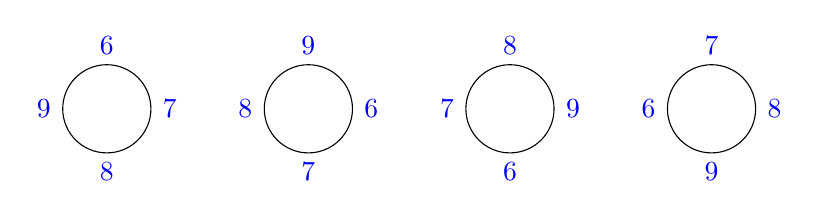
\begin{tikzpicture}[scale=0.8]
  \foreach \k/\a/\b/\c/\d in {0/6/7/8/9,1/9/6/7/8,2/8/9/6/7,3/7/8/9/6} {
    \begin{scope}[xshift=\k*3.2cm]
      \draw (0,0) circle (0.7);
      \node[blue] at (0,1) {$\a$}; \node[blue] at (1,0) {$\b$};
      \node[blue] at (0,-1) {$\c$}; \node[blue] at (-1,0) {$\d$};
    \end{scope}
  }
\end{tikzpicture}
\end{center}

ដូច្នេះ ចំពោះចម្លាស់ជាវង់មួយរបៀបនេះអាចយកមករៀបជាចម្លាស់ជាជួរដេកបាន $4$ របៀបខុសគ្នា ។ គេបានចំនួនចម្លាស់វង់តិចជាងចំនួនចម្លាស់ជាជួរដេក $4$ ដង ។ ដោយចំនួនចម្លាស់នៃ $4$ ធាតុជាជួរដេកមាន $4!$ នោះចំនួនចម្លាស់វង់នៃ $4$ ធាតុមាន $\dfrac{4!}{4} = \dfrac{4\cdot 3!}{4} = 3! = 3\cdot 2\cdot 1 = 6$ របៀប ។

\begin{formulaBox}[ជាទូទៅ]
ចំនួនចម្លាស់វង់នៃ $n$ ធាតុគឺ $\dfrac{n!}{n} = (n - 1)!$ ។
\end{formulaBox}

\begin{example}[លំហាត់គំរូ]
គ្រួសារមួយមានមនុស្សចាស់ $4$ នាក់ និងក្មេង $2$ នាក់អង្គុយហូបបាយជុំវិញតុមូលមួយ ។
\begin{enumerate}[a]
  \item តើការអង្គុយនេះមានប៉ុន្មានរបៀបខុសគ្នា ។
  \item បើក្មេង $2$ នាក់អង្គុយជិតគ្នាជានិច្ច តើការអង្គុយនេះមានប៉ុន្មានរបៀប?
\end{enumerate}
\end{example}
\ans
\begin{enumerate}[a]
  \item របៀបអង្គុយរបស់មនុស្ស $6$ នាក់នេះជាចម្លាស់វង់នៃ $6$ ធាតុ ។ ចំនួនចម្លាស់វង់នៃ $6$ ធាតុគឺ $\dfrac{6!}{6} = 5! = 5\times 4\times 3\times 2 = 120$ របៀប ។
  \item បើមានក្មេងពីរនាក់អង្គុយជិតគ្នា នោះយើងគិតថាក្មេង $2$ នាក់នេះអង្គុយរួមគ្នាមួយកន្លែងដូច្នេះ ជាចម្លាស់វង់ $5$ ធាតុ ប៉ុន្តែរបៀបដែលក្មេងទាំងពីរអង្គុយជិតគ្នាមាន $2$ របៀបផ្សេងគ្នា (ឆ្វេង ឬស្ដាំគ្នា) ។ ចំនួនចម្លាស់វង់ដែលក្មេង $2$ នាក់អង្គុយជាប់គ្នាមានចំនួន $2!(5 - 1)! = 2\times 4! = 2\times 4\times 3\times 2 = 48$ របៀប ។
\end{enumerate}

\begin{pro}
សិស្សមួយក្រុមមានស្រី $2$ នាក់ ប្រុស $6$ នាក់អង្គុយជុំវិញតុមូលធ្វើការងារជាក្រុម ។ តើសិស្សអាចអង្គុយបានប៉ុន្មានរបៀប បើសិស្សស្រី $2$ នាក់អង្គុយទល់មុខគ្នា ។
\ans
$6! = 720$ ។
\end{pro}

\section*{លំហាត់អនុវត្តន៍}
\begin{enumerate}[1]
  \item គេបោះគ្រាប់ឡុកឡាក់ $2$ គ្រាប់ខុសគ្នា ។ រកចំនួនលទ្ធផលដែលអាចកើតឡើង បើផលបូកគ្រាប់ឡុកឡាក់ស្មើនឹង $8$ ឬ $9$ ។
  \ans
  ផលបូក $8$ មាន $5$ លទ្ធផល ហើយផលបូក $9$ មាន $4$ លទ្ធផល ។ ដូច្នេះ $5 + 4 = 9$ ។
  \item គេមានរថយន្តឈ្នួល $3$ ប្រភេទសម្រាប់បំរើសេវាធ្វើដំណើរទៅឬមកពីក្នុងភូមិនៅទីប្រជុំជនមួយដែលនៅក្បែរគ្នា ។ ពេលធ្វើដំណើរទៅទីប្រជុំជន ពូសុខអាចជិះរថយន្តណាមួយ ឬក៏គាត់ដើរដោយខ្លួនឯង ។ ហេតុនេះ ពេលត្រឡប់មកផ្ទះវិញ គាត់សម្រេចចិត្តថាជិះរថយន្ត ។ តើការធ្វើដំណើរទៅនិងត្រឡប់មករបស់គាត់មានប៉ុន្មានរបៀប?
  \ans
  ទៅមាន $3 + 1 = 4$ របៀប មកវិញមាន $3$ របៀប ៖ $4\times 3 = 12$ ។
  \item មានបុរស $6$ នាក់ និងនារី $5$ នាក់ចាប់ដៃគូគ្នារាំវង់ ។ តើការចាប់ដៃគូស្រីប្រុសនេះមានប៉ុន្មានរបៀប?
  \ans
  $6\times 5 = 30$ ។
  \item នៅថ្ងៃសម្រាកមួយ សុភីរៀបផែនការការងាររបស់ខ្លួន ធ្វើកិច្ចការសាលារៀន បោកសម្លៀកបំពាក់ អានកាសែត ទស្សនាវដ្ដី និងស្រាវជ្រាវឯកសារតាមអ៊ីនធឺណែត ។ តើសុភីអាចរៀបផែនការរបស់ខ្លួនបានប៉ុន្មានរបៀប?
  \ans
  $4! = 24$ ។
  \item រកចំនួនទាំងអស់នៃចំនួនដែលមានលេខ $4$ ខ្ទង់ដោយប្រើគ្រប់លេខរបស់ចំនួន $4129$ ។
  \ans
  $4! = 24$ ។
  \item ថ្នាក់រៀនមួយមានសិស្ស $40$ នាក់ គ្រូត្រូវការសិស្ស $2$ នាក់ដើម្បីឡើងដោះស្រាយលំហាត់លេខ $2$ និងលេខ $5$ ដែលមាននៅក្នុងសៀវភៅលំហាត់ ។ តើគ្រូអាចហៅសិស្សបានប៉ុន្មានរបៀបដើម្បីដោះស្រាយលំហាត់?
  \ans
  ${}_{40}P_2 = 40\times 39 = 1560$ ។
  \item តើជ័យលាភីមានចំនួនប៉ុន្មានរបៀប ដើម្បីចាប់យករង្វាន់លេខ $1$ លេខ $2$ និងលេខ $3$ សម្រាប់មនុស្ស $9$ នាក់ ។
  \ans
  ${}_9P_3 = 504$ ។
  \item កាក់មួយមានមុខពីរគឺខាងរូប និងខាងលេខ ។ គេបោះកាក់នេះ $4$ ដងបន្តបន្ទាប់គ្នា ។ រកចំនួនលទ្ធផលដែលអាចកើតឡើងទាំងអស់ ។ សង់ដ្យាក្រាមដើមឈើ ។
  \ans
  $2^4 = 16$ ។
  \item កុមារវិនយកឃ្លី $6$ ពណ៌ផ្សេងៗរៀបជារង្វង់ឱ្យឆ្លាស់ពណ៌គ្នា ។ តើវិនអាចរៀបបានប៉ុន្មានរបៀបផ្សេងៗគ្នា ។
  \ans
  $(6 - 1)! = 120$ ។
  \item គណនា ៖
  \begin{enumerate}[a]
    \item $\dfrac{4!}{3!}$, $\dfrac{10!}{7!}$, $\dfrac{9!}{5!3!}$, $\dfrac{(n - 1)!}{n!}$, $\dfrac{n!}{(n - 3)!}$, $\dfrac{(n!)^2}{(n - 1)!(n - 2)!}$
    \item ${}_6P_4$, ${}_5P_3$, ${}_7P_7$ ។
  \end{enumerate}
  \ans
  ក. $4$; $720$; $504$; $\dfrac{1}{n}$; $n(n - 1)(n - 2)$; $n^2(n - 1)$ \quad ខ. $360$; $60$; $5040$ ។
  \item ចំពោះ $n \in \mathbb{N}$ ចូរដោះស្រាយសមីការ ៖
  \begin{tasks}(5)
    \task ${}_nP_3 = 60$
    \task ${}_nP_2 = 56$
    \task ${}_nP_2 = 30$
    \task ${}_nP_3 = 990$
    \task ${}_6P_r = 30$
  \end{tasks}
  \ans
  ក. $n = 5$ \quad ខ. $n = 8$ \quad គ. $n = 6$ \quad ឃ. $n = 11$ \quad ង. $r = 2$ ។
  \item រោងភាពយន្តមួយ ត្រូវបញ្ចាំងខ្សែភាពយន្ត $4$ រឿងខុសៗគ្នាក្នុង $1$ ថ្ងៃ ។ តើគេអាចរើសខ្សែភាពយន្ត $4$ រឿងមកបញ្ចាំង ក្នុងចំណោមខ្សែភាពយន្ត $11$ រឿងបានប៉ុន្មានរបៀប?
  \ans
  ${}_{11}P_4 = 7920$ (គិតលំដាប់ម៉ោងបញ្ចាំង) ។
  \item ប៉ុស្តិ៍នគរបាលមួយមានគ្នា $5$ នាក់ និងមានសំណុំរឿងឧក្រិដ្ឋចំនួន $7$ ករណី ។ តើមានប៉ុន្មានរបៀបដែលនគរបាលម្នាក់ ត្រូវសើបអង្កេតសំណុំរឿងឧក្រិដ្ឋ $1$ ករណីផ្សេងៗគ្នា?
  \ans
  ${}_7P_5 = 2520$ ។
  \item តើគេអាចរើសសន្លឹកឆ្នោត $4$ សន្លឹកពីសន្លឹកឆ្នោត $50$ សន្លឹកបានប៉ុន្មានរបៀប ដើម្បីឱ្យសន្លឹកឆ្នោតនីមួយៗឈ្នះរង្វាន់ផ្សេងៗគ្នា?
  \ans
  ${}_{50}P_4 = 5\,527\,200$ ។
  \item តើគេអាចបង្កើតប័ណ្ណសម្គាល់ខ្លួនដែលមាន $6$ ខ្ទង់បានប៉ុន្មានរបៀបដោយលេខតាមខ្ទង់នីមួយៗប្រើបានតែមួយដងប៉ុណ្ណោះ?
  \ans
  ${}_{10}P_6 = 151\,200$ ។
\end{enumerate}
